\documentclass[border=10pt]{standalone}
\usepackage{tikz}
\usepackage{etoolbox}
\makeatletter
\patchcmd\pgfpatharc{\pgfutil@in@}{%
  \pgfmathiftrigonometricusesdeg{}{%
%    \typeout{\pgf@temp@a, \pgf@temp@b}%
    \pgfmathradians@{\pgf@temp@a}\let\pgf@temp@a\pgfmathresult
    \pgfmathradians@{\pgf@temp@b}\let\pgf@temp@b\pgfmathresult
%    \typeout{\pgf@temp@a, \pgf@temp@b}%
    \def\pgfmath@trig@format@choice{0}% \pgfset{trig format=deg}
  }\pgfutil@in@}{}{\PatchFailed}
\makeatother
\begin{document}
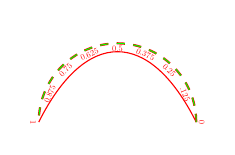
\begin{tikzpicture}
\draw[trig format=rad, red]  (0:1) arc(0:pi:1) % check if timer is correct:
  node foreach \p in {0,.125,...,1} [pos=\p, sloped, scale=.3, below] {\p};
\draw[red, dashed, thick] (0:1) arc(0:pi r:1);
\draw[green, dashed] (0:1) arc[start angle=0, end angle=pi r, radius=1];
\end{tikzpicture}
\end{document}